%% LyX 2.1.0 created this file.  For more info, see http://www.lyx.org/.
%% Do not edit unless you really know what you are doing.
\documentclass[12pt,english]{svjour3}
\usepackage[T1]{fontenc}
\usepackage[latin9]{inputenc}
\usepackage{geometry}
\geometry{verbose}
\usepackage{url}
\usepackage{graphicx}
\usepackage[authoryear]{natbib}

\makeatletter

%%%%%%%%%%%%%%%%%%%%%%%%%%%%%% LyX specific LaTeX commands.
%% Because html converters don't know tabularnewline
\providecommand{\tabularnewline}{\\}

\makeatother

\usepackage{babel}
\begin{document}

\title{Fertility, Household Labor Supply and Agricultural Production}


\subtitle{Instrumental Variable Evidence from Uganda}


\titlerunning{Fertility, Household Labor Supply and Agricultural Production}


\author{Bjorn Van Campenhout}


\institute{International Food Policy Research Institute (IFPRI) - Kampala -
Plot 15, East Naguru Road, Po Box 28565 - Kampala - Uganda - b.vancampenhout@cgiar.org
- +256 790 833729}


\authorrunning{Bjorn Van Campenhout}

\maketitle
Keywords: fertility, instrumental variables, household labour supply,
agriculture, Uganda.

JEL codes: J13, J22, Q12
\begin{abstract}
Fertility is likely to affect agricultural production through its
effect on household labor supply. Using the fact that in traditional,
patriarchal societies sons are preferred to girls, we isolate exogenous
variation in the number of children born to the mother and related
it to labor supply and production outcomes in Uganda, a country that
combines a dominant agricultural sector with one of the highest fertility
rates in the world. We find that fertility has a strong negative effect
on hours worked by the mother in the field. We also find some evidence
of a negative effect for the father, but the size of the effect is
only half that of the women. There is no effect on child labour. Households
with lower fertility devote significantly more time to land preparation
and weeding. This results in the fact that larger households grow
less matooke and sweet potatoes. 
\end{abstract}

\section{Introduction}

At the most basic level, subsistence farmers in rural Africa combine
natural with human resources to make a living. They use mainly household
labor on their own small plots to produce for own consumption. As
such, the quantity of family labor available is an important determinant
of well-being. Family labor availability, generally believed to suffer
much less from moral hazard problems, will be a direct function of
the number of biological children within the household. For instance,
more children means more hands to work on the field. At the same time,
more children means mothers, and to a lesser extend siblings and fathers,
will need to spend more time on reproductive chores meaning less time
will be available to spend on agricultural activities. Since women
are known to supply most of the agricultural labour the loss in time
needed for reproductive activities potentially offsets the the gains
from larger families. 

Uganda has one of the highest fertility rates in the world and a substantial
part of the population lives in rural areas making a living out of
semi-subsistence agriculture. Even in the context of large reductions
in child mortality rates, total fertility rates remain stubbornly
high. On average, Ugandan women in rural areas bear 6.8 children over
the course of their reproductive lives \citep{New9}. The question
on how fertility affects well-being through its effect on household
labour supply and agricultural production is therefore relevant. For
example, knowledge on how fertility affects time allocation by different
categories within the household is important to gender-stream efforts
related to crop intensification and commercialization.

In this study, we will investigate the effect of fertility on agricultural
production at the household level. In particular, we will investigate
the effect of the number of biological children on household member
labor input. We will also look at the effect of fertility on crop
portfolio, area cultivated, production and productivity for the five
most important crops. However, fertility is a choice variable to agricultural
households. For instance, mothers who work long hours in the field
may try to avoid becoming pregnant because this would only increase
hardship. Or, households with low agricultural production may deliberately
choose to have more children because this means cheap labor. If fertility,
time allocations and agricultural production is indeed jointly determined,
just looking at correlations will be misleading, and one needs to
find a way to separate the exogenous variation from the part that
is jointly determined.

Our identification strategy is a simple but powerful instrumental
variables approach inspired by the work of \citet{RePEc:aea:aecrev:v:88:y:1998:i:3:p:450-77}.
We use the fact that male off-springs are preferred in conservative,
patriarchal societies to construct a range of instruments. The exogenous
variation in the sex of a child can then be used to determine the
exogenous component of household size. Such a two stage least squares
approach is expected to yield consistent estimates for the causal
effect of fertility on agricultural labor supply and associated agricultural
production within the household.

There is an active debate among scholars in the field of labour economists
on the relationship between fertility and labour supply. \citet{RePEc:aea:aecrev:v:88:y:1998:i:3:p:450-77}
use the fact that American couples prefer children of different sex,
and and are likely to keep trying if the first two children are of
the same sex as a source of exogenous variation. We will argue that
in a developing country context, the sex of the (first born) child
makes more sense as an instrument. Indeed, this instrumentation strategy
has been used in such a context. \citet{doi:10.1080/00220380500356779}
use the sex of the first two children to predict exogenous variation
in fertility in India and its effect on well-being. We feel it is
too ambitious to relate fertility directly to poverty and related
measures of consumption as there may be ways in which the instrument
can affect consumption besides through the fertility channel. We therefore
restrict ourselves to labour allocation, area planted and production.
In addition, most studies that look at the effects of fertility on
labour allocation are on data from Asia. Well documented high incidence
of selective abortion in these areas means the sex of the first child
or children becomes endogenous as well. This is likely to be much
less of a problem in our application, which is to our knowledge the
first such application to an African country.

We find that the sex of the first-born, the sex of the first two children
born, as well as the percentage of girls a a share of total children
in each age cohort all significantly explain observed fertility, measured
as the gap between actual children born and a theoretical maximal
fecundity for each age cohort. Fertility has a strong negative effect
on hours worked by the mother in the field. We also find some evidence
of a negative effect for the father, but the size of the effect is
only half that of the women. There is no effect on child labour. Households
with lower fertility devote significantly more time to land preparation
and weeding. We also find that smaller households grow and produce
more matooke. This effect holds to a lesser extent for sweet potatoes.
We find no impact on yields. 

This article is organized as follows. The next section gives a brief
overview of the most prominent papers that are related to the present
paper. Then, we make our case for the use of the sex of the first-born
as an instrument using literature that documents child gender and
reproductive behaviour. We then present the data we will use in our
application, and describe our main variables we will use in the analysis.
Next, we present the results. In this section, we first take a close
look at the first stage regression. We then look at the effect of
fertility on household labor supply, considering differential effects
depending on household demographics as well as agricultural labor
activities. We then turn to the effect of household size on productivity.
A final section concludes.


\section*{Related Studies}

Fertility and the related concept of household size impacts household
well-being trough consumption and production. \citet{RePEc:ecj:econjl:v:105:y:1995:i:433:p:1415-34}
focus more on the consumption side effects of household size in a
developing country context. They note the contradiction between widely
held views that larger households are often poorer (due to increased
competition for a given food stock) and scale economies in consumption.
The find that, if economies of scale are accounted for within households,
the negative correlation between household size and consumption expenditure
disappears. On the production side of the farm household, the effect
of household size is equally ambiguous. Some may argue that larger
households means that more labor is available within the household.
The additional advantage of this labor is that it is not subject to
the moral hazard effects often attributed to hired labor%
\footnote{For instance, \citet{RePEc:eee:deveco:v:18:y:1985:i:2-3:p:297-313}
argues this may the reason why small farms appear to be more efficient
than large farms%
}. But at the same time, more dependents within the household means
more time needs to be allocated to reproductive activities. Also,
agricultural labour and agricultural production may be subject to
diminishing returns. In this study, we will start by investigating
the link between fertility and agricultural labour supply and then
look at the relation between fertility and agricultural production
respectively.

The relationship between fertility and household labor supply has
been studied most carefully in the field of labor economics. Since
this literature is so extensive, we only mention two of the most influential
works here. The first is \citet{RePEc:aea:aecrev:v:88:y:1998:i:3:p:450-77},
who attempt to quantify the effect of fertility on labor supply in
the US. They deal with the endogeneity of the number of children women
have by exploiting the fact that Americans tend to prefer mixed sibling-sex
in their household. They argue that parents of same-sex siblings are
significantly and substantially more likely to go on to have an additional
child. They find that more children does indeed reduce labor force
participation of women, but the effect is less pronounced than previous
studies suggested. They find no effect on the labour supply of the
father.

Another paper that tries to answer the same question is \citet{RePEc:ucp:jpolec:v:88:y:1980:i:2:p:328-48}.
In this paper, the exogenous variation in the number of children is
obtained by using the occurrence of multiple births (twins) at first
birth as an instrument. The authors argue that the comparison between
women who gave birth to a single child at first birth and women who
gave birth to twins at first birth teases out the causal effect of
related to an extra child. Since the occurrence of twins is exogenous,
there is no danger that heterogeneity in women preferences contaminates
the estimated coefficients. The study finds that household size reduces
female labor supply, but the effect is only temporary%
\footnote{In addition to studies that investigate the causal effect of household
size on (female) labor supply, there are also a range of papers that
test Becker's quantity-quality fertility model \citep{RePEc:nbr:nberch:2387,RePEc:ucp:jpolec:v:81:y:1973:i:2:p:s279-88}.
Many of these articles also use twins \citep{RePEc:ecm:emetrp:v:48:y:1980:i:1:p:227-40,RePEc:tpr:qjecon:v:120:y:2005:i:2:p:669-700}
and/or sibling sex composition \citep{New1,RePEc:ucp:jlabec:v:28:y:2010:i:4:p:773-824}.%
}.

\citet{doi:10.1080/00220380500356779} use sex of the first two children
as a natural experiment and find that household size has a positive
effect on poverty in India. They use essentially the same argument
as we will make in the next section. Our study, however, is are less
ambitious. We feel that there are too many pathways through which
household size can influence poverty to be useful. In addition, welfare,
and the related concept of poverty, relies on consumption per capita.
Consumption per capita as the independent variable is likely to be
problematic in the two stage least squares setting. There is a real
danger that the instrumental variable affects the outcome variable
directly, instead of only through its influence in family size. For
instance, if boys consume on average more than girls, the exclusion
restriction is violated. They confirm that high fertility is correlated
with poverty, but the correlation disappears when they account for
potential endogeneity of fertility. There is also some evidence on
Indonesia. \citet{RePEc:dem:demres:v:20:y:2009:i:26} looks at the
relation between consumption and fertility. In \citet{RePEc:iza:izadps:dp2162},
fertility is related to the allocation of labour within households.
However, they move away from the direct instrumental variable approach
that is standard and instead estimate a reproduction function taking
into account endogenous contraceptive choice. 

All the above studies employ data from South East Asia. It is well-known
that fertility at birth is already skewed in many Asian countries.
For instance India, from which \citet{doi:10.1080/00220380500356779}
drawn their sample, is particularly known for selective abortion of
girls \citep{New8}. This suggests a relationship between the instrument
and the error term of the structural equation. It is well know that,
in the context of weak instruments, such correlation can seriously
bias estimates \citep{1995}. The likely negative correlation between
the instrument and the error term will mean that, in this case, \citet{doi:10.1080/00220380500356779}'s
estimates are biased downward, in the direction of their original
OLS estimate. This bias is likely to be much less pronounced in our
data.

In our paper, we will try to address some of the above challenges.
We will use the sex of the first-born and variations thereof as our
instrumental variables. We will relate fertility to agricultural labour
supply and agricultural production, since there is a direct link between
these three variables. We will also concentrate on Africa. Here, while
there is a boy preference, reproduction rate norms are high and the
cost of raising children is low. This means that selective abortion
is much less of a concern. Still, we rely on the sex and numbers of
children within the family, meaning that the kind of sex preference
as described in \citet{Jayachandran01082011} may still render our
instrument endogenous.


\section*{Boy preference and Fertility}

There is quite some evidence that parents prefer boys over girls in
developing countries%
\footnote{In developed countries, there is a preference for a mix of sexes among
children, as shown in, for example \citet{RePEc:aea:aecrev:v:88:y:1998:i:3:p:450-77}.%
}. For instance there is a large body of literature that looks at correlations
between sex and variables related to well-being or quality of children.
Significant differences in these outcomes are then considered proof
of sex bias. \citet{New5} and \citet{New6} look at excess mortality
among female infants. \citet{New7} and \citet{testit} investigate
differential access to health. \citet{RePEc:oup:oxecpp:v:40:y:1988:i:1:p:32-54}
and \citet{doi:10.1080/713600059} find a correlation between sex
and nutrition and \citet{RePEc:ucp:jpolec:v:90:y:1982:i:1:p:52-73},
\citet{RePEc:ier:iecrev:v:36:y:1995:i:3:p:795-818} and \citet{RePEc:eee:streco:v:9:y:1998:i:4:p:453-468}
all investigate correlations between the gender of children and education.

However, at a more basic level, boy preference is already revealed
by parents who, if asked in for example surveys, state clearly that
they want to have more boys than girls. Such preferences lead to a
particular decision rule with respect to fertility, where the likelihood
that children are added to the household is positively correlated
to the number of surviving girls in the household. The preference
for a boy over a girl results in what \citet{Jayachandran01082011}
refer to as a stop-after-a-son fertility pattern. There are many studies
that show empirically that in settings with son preference, a couple
that just had a son is more likely to stop having children \citep{RePEc:spr:demogr:v:24:y:1987:i:4:p:517-530}
or wait longer to have the next child \citep{RePEc:spr:demogr:v:22:y:1985:i:2:p:145-168,New4,RePEc:spr:demogr:v:37:y:2000:i:1:p:95-108,RePEc:bla:popdev:v:27:y:2001:i:1:p:33-63}. 

\citet{Jayachandran01082011} argue that son preference leads mothers
to breastfeed daughters and children without brothers relatively less
long. This underlying consequence of sex bias my partly explain a
range of outcomes observed in the area of health, mortality and possibly
even educational attainment. Their model shows that even when parents
want both boys and girls to have the same health and education, disparities
can arise passively because of fertility preferences. They show that
a ``try until you have a boy'' fertility rule results in girls having
on average more siblings, leading to more competition for resources
within the household. 

The use of the sex of first born as an instrument is motivated by
various cultural and economic factors documented in the anthropological
and demographic literature. In countries where no old age insurance
is available, parents may choose to invest more in children that have
a higher chance of being able to support them at old age \citep{RePEc:ucp:jpolec:v:90:y:1982:i:1:p:52-73}.
Anthropological and demographic evidence emphasize the dominant role
of males in traditional patrilineal societies where descent and inheritance
are transmitted through the male line. Furthermore, male children
strengthen the relationship between the wife and her husband's kin
(by guaranteeing the continuation of his lineage) and secure (the
mother's) access to residence and inheritance upon the husband's death.
Also, the practice of dowry implies that a daughter is often associated
with an expected expenditure, a central part in the theoretical model
of son preference in \citet{doi:10.1080/00220380500356779}. 

Most of the evidence on boy preference comes from Asian countries.
It is often assumed that gender preferences are much lower or even
absent in Sub-Saharan Africa. This is surprising, as many of the cultural
and economic factors that are observed in Asia equally apply to Africa.
One study that documents significant gender bias in Africa is \citet{RePEc:oup:restud:v:77:y:2010:i:4:p:1262-1300},
who find skewed sex ratios at older age in favor of men. What is different
from the Asian context, though, is that the vast majority of women
are not missing at birth, but throughout the entire age spectrum%
\footnote{The large effects documented in \citet{RePEc:oup:restud:v:77:y:2010:i:4:p:1262-1300}
have recently been attenuated in \citet{RePEc:got:gotcrc:133}, who
confirm only missing young adult women.%
}. \citet{New3} argues that gender bias is likely not to be found
at birth in the African context where high fertility is culturally
valued and made less costly for families that still rely on the support
from the extended family system. In Uganda, preference for boys has
been documented in \citet{New2}.

Even in Western societies, preference for the firstborn to be a son
has been observed. For example, \citet{test} report an extensive
list of studies that find men and/or women prefer a boy rather than
a girl as their first-born. Even in the United States, the \citet{RePEc:aea:aecrev:v:88:y:1998:i:3:p:450-77}
provides some evidence of an association between having a male child
and reduced childbearing at higher parities, in addition to the mixed-child
preference. As such, we feel that the sex of the first-born (or closely
related indicators) provide a valid instrument for fertility at the
household level.


\section*{Data and Descriptive Statistics}

We will use the Uganda National Household Survey (UNHS) 2005/06. While
being somewhat dated, we have chosen this survey because it has much
more information on agriculture than the more recent UNHS of 2009/10.
Structured with a standard Living Standard Measurement Survey - Integrated
Survey on Agriculture (LSMS-ISA) in mind, the UNHS 2005/06 collected
detailed information on a sample of almost 43000 people in 7500 households
in Uganda.

Ideally, we would like to have a sample of households where all desired
children where born. A household that currently has one child may
be in the process of adding more children to their family. Assume
a couple that has just formed and is entering their reproductive stage.
Assume further that the first child is a girl. In our sample, this
household will show up with a smaller than average size, but with
a girl as the firstborn, hence this may mistakenly be interpreted
as running against our hypothesis that households prefer boys. If
the first child is a boy, this same household would show up in our
sample as smaller than average, and thus this may lead us to put too
much confidence in our hypothesis. The fact that we are working with
a cross section of households rather than historical data on all births
by women that have reached the end of their reproductive lives is
also reflected in the average number of children. This is only 3.13
children, while women bear almost 7 children over their entire reproductive
period. 

To deal with this problem, we work with the difference in the actual
number of children reported and the maximum reproductive capacity
for a woman at a certain age, rather than simply the number of children
in the household%
\footnote{Alternatively, one could use the number of children within the household
and control for the age of the mother. We have also run the analysis
using this strategy and got the same conclusions. %
}. We will refer to this measure of fertility as the gap or shortfall
in fertility. To get the latter, we would need to estimate the average
age at menarche within the population, and then simply divide into
age the pregnancy period plus post pregnancy lactation in-fecund period.
In addition, one would also need to corporate the maternal mortality
ratio for \textquotedbl{}censoring\textquotedbl{} women's lives who
have too many children and thus increasing her mortality rate (and
exit from the sample). However, we took the 95th percentile of total
fertility rates per age from the Demographic and Health Survey of
Uganda (2011). This is probably a good approximation of the upper
bound by age of fertility in the population.

The selection of children is base on the household roster. In particular,
we will select individuals that respond they are son or daughter of
the household head. There is a potential problem when using a cross
sectional survey such as the UNHS that only looks at reported dependents
currently living within the household to calculate the difference
between actual and theoretical fertility. Older women may be living
in households where some of the older children have already left the
household. Thus, at around the age of thirty, the gap between reported
children in the household and theoretical fertility starts to increase
more rapidly because of children growing old enough to start household
of their own. More troubling, the reported gender of the oldest son
or daughter living in the household may not be the gender of first-born.
To overcome this problem, we restrict our sample to households where
the mother is between 16 and 32. The cut off age of 32 is because
at this age, the first-born of the mother will turn 16, which is our
entry age into the sample of mothers.

Looking at the sex of the first-born is only one possible strategy.
One may argue that the sex of the first born is not very relevant
in a context where women bear on average almost 7 children. Indeed,
it is likely that households will get a second child irrespective
of the sex of the first. This is supported by \citet{Jayachandran01082011},
who find that the difference in breastfeeding duration between boys
and girls is largest near target family size, when gender is most
predictive of subsequent fertility. Therefore, we will not only use
the sex of the firstborn child as an instrument for fertility, but
also experiment with alternative instruments such as an indicator
that the first two children are girls or a variable that expresses
the share of female children in the total family size.


\subsubsection*{Fertility}

In this section, we will present some descriptive statistics to check
if boy preference is reflected in fertility patterns in the Ugandan
data. Table \ref{tab:gender-and-fertility} summarizes our findings.
The first two columns checks if households that have a daughter as
first-born are more likely to have extra children. We simply calculated
the percentage of households that had more than one child conditional
on their first born being a son or a girl. We find that in the sub-sample
where the first child is a boy, about 37.46 percent of households
will have at least one more child. However, if the first child happened
to be a girl, almost 40 percent of households will have at least one
more child. 

We also look at the shortfall in actual fertility to theoretical fertility.
In the first two columns, we report this fertility gap for two groups
of households. We find that households that have a boy as the firstborn
child have an average fertility gap of about 2.46 children. Consistent
with the proposition that have a firstborn girl are likely to have
more children conditional on age, we find that the gap is smaller
then the firstborn is a girl (2.26). In other words, households where
the firstborn is a girl will be closer to the theoretical maximal
fertility than those that had a boy as the firstborn. The difference
in the fertility gap between the group of households with a first
born boy and a first born girl is significant (p=0.003).

The third and fourth column present the same statistics, but now looks
the sex of the first two children. As such, there are three possible
scenarios. If the first two children are both boys, we expect that
the chance that they have extra children is lowest. We find the probability
of adding children in this case to be just over 13 percent. If the
first was a girl and the second was also a girl, we expect there is
a higher chance that parents choose to have extra children. In this
case, there is an almost 14 percent chance that they add at least
one child to the household. For those that had a first girl but their
second child was a boy, we expect the probability of increasing household
size to lie between the two, which is indeed the case. The lower panel
shows that the gap between actual and potential household size is
largest when the first two children are boys. The gap is smallest
when the first two children are both girls.

Finally, we compare the average fertility in two different groups
defined by the share of female children within the total number of
children. As already stated above, because of boy preference, female
children are likely to live in larger families. We indeed find that
if there are more girls than boys amongst the children, the average
number of children is higher. We also find a difference in the fertility
gap that is significant with associated p-value of 0.021.

\begin{table}
\protect\caption{gender and fertility\label{tab:gender-and-fertility}}


\centering{}%
\begin{tabular}{cccccc}
\hline 
 & prob +1 &  & prob +1 &  & av fertility\tabularnewline
\hline 
1st=boy & 0.375 & 1st=boy, 2nd=boy & 0.132  & \% daughters<0.5 & 2.78\tabularnewline
1st=girl & 0.393 & 1st=girl, 2nd=boy & 0.134 & \% daughters>0.5 & 2.88\tabularnewline
 &  & 1st=girl, 2nd=girl & 0.139 &  & \tabularnewline
\hline 
 & gap &  & gap &  & gap\tabularnewline
\hline 
1st=boy & 2.46 & 1st=boy, 2nd=boy & 2.46 & \% daughters<0.5 & 2.41\tabularnewline
1st=girl & 2.26 & 1st=girl, 2nd=boy & 2.38 & \% daughters>0.5 & 2.32\tabularnewline
 &  & 1st=girl, 2nd=girl & 2.06 &  & \tabularnewline
\hline 
\end{tabular}
\end{table}



\subsubsection*{Hours worked }

In this section we will briefly look at some descriptive statistics
on labor supply, one of the prime pathways through which fertility
affects productivity and well-being. Most of Uganda has two cropping
seasons. The first runs from January to June. The second cropping
season is from July to December. The UNHS 2005/06 interviewed households
twice over the course of one year to capture this feature. It visited
households in the beginning of 2005 to capture the second cropping
season in 2004 (that is, running from July to December 2004). Households
were revisited at the end on 2005 to record information from the first
cropping season in 2005 (running from January to June 2005). In our
study, we will only consider the 2004 cropping season, as data for
labour allocation to agriculture was unavailable for the 2004 cropping
season.

Figure \ref{fig:Average-hours-worked} shows time reported on the
field along different dimensions%
\footnote{The dimensions are mother, father or child; land preparation, input
application, weeding and harvesting; and crop. The crops are the five
most grown crops.%
}. One of the most obvious observations is that women do most of the
work, and child labor is restricted to about one day per crop and
activity during the entire season. This already indicates that the
trade-off between the time lost by the mother because of rearing the
children and the time gained by extra hands is likely to work against
agricultural production. Typical for Uganda is the low amount of time
spent on applying inputs. Farmers in Uganda use very limited amounts
of fertilizer and other inputs, so also the time spend on applying
them is small. There is also some heterogeneity in the time spend
on different crops. For instance, matooke requires less time than
maize, both for men and for women. However, there are also difference
between the sexes. For instance, women spend much more time cultivating
sweet potatoes, and to a lesser extent beans, than men. 

\begin{figure}
\protect\caption{Average hours worked\label{fig:Average-hours-worked}}


\centering{}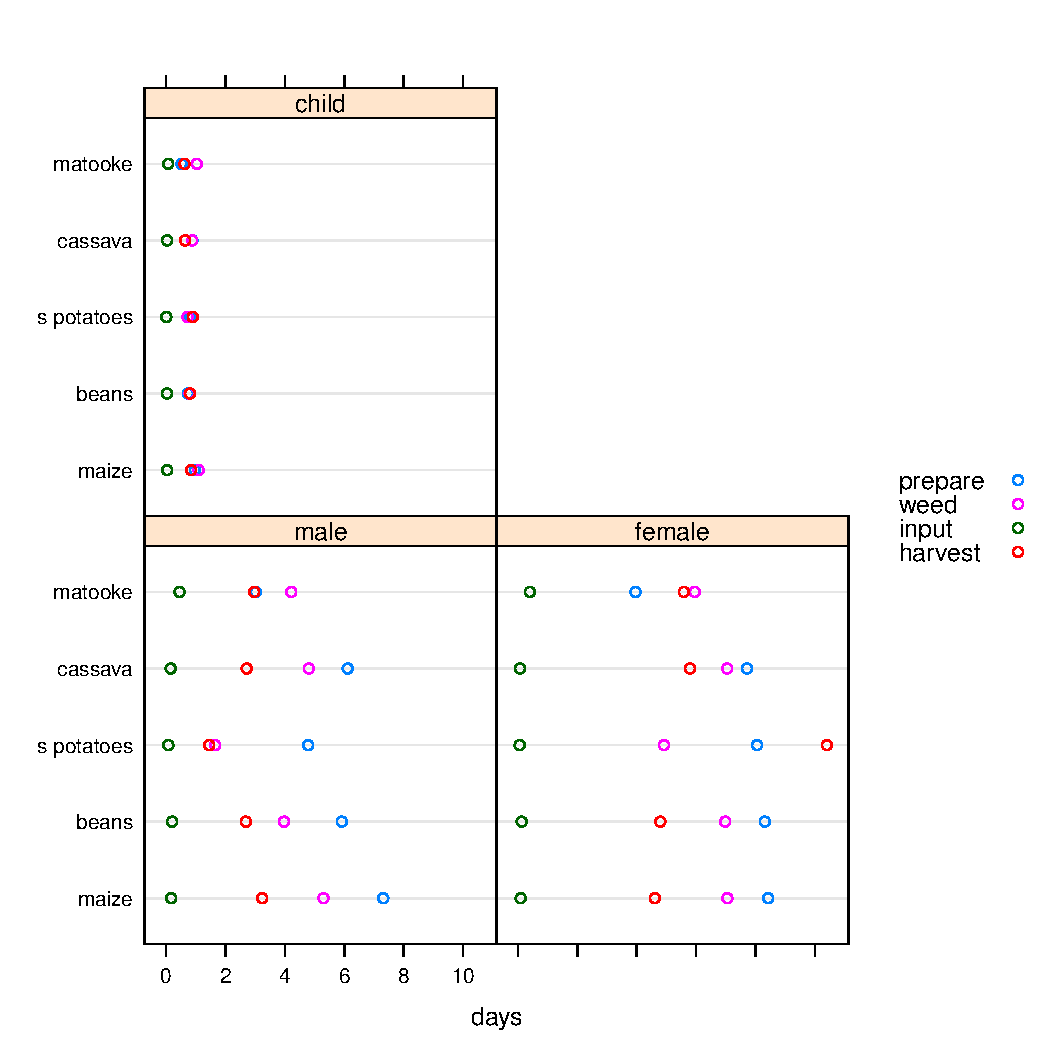
\includegraphics[scale=0.6]{dotplot}
\end{figure}



\subsubsection*{Production\label{sub:Production}}

We also investigate the effect of fertility on production of some
of the most important crops. More in particular, we look at the effect
of fertility on the likelihood that a household cultivates each of
the five most important crops. The first row in table \ref{tab:2averages}
reports on the percentage of households that grow each of the crops.
Over 50 percent report growing maize, beans and cassava. We also look
at the impact on area cultivated, measured in acres. Households on
average allocate about half an acre to maize. The least space is reserved
for sweet potatoes. We also express area cultivated as a share of
total area under cultivation. We find that about 17 percent of total
land area is allocated to maize. The next line reports average production
in kilograms at the household level. This may seem low, but this because
households that report not to produce the crop are also part of the
average. We also divide by household size. Finally, we report yields
for the five crops, defined as the amount of each crop harvested per
unit of land (per acre).

We also aggregate the different corps by weighing them to average
prices. We use prices from FoodNet. In particular, we average prices
observed in Kampala's Nakawa market over the July to December 2004
period. Doing so, we find that the average total value derived from
these five crops is about UGX98,500, which translates to about UGX45000
per capita. About 40 percent of the households in their reproductive
age does not cultivate any of these five crops. On average, about
0.69 acres is allocated to these five crops. The yield per acre is
about UGX220,220.

\begin{table}
\protect\caption{Averages\label{tab:2averages}}


\begin{tabular}{rcccccc} \hline \hline
	&	maize	&	beans	&	s potatoes	&	cassava		&	matooke	

\\

\hline

% growing crop    &      59.1  &      52.6 &     38.8  &      51.8 &      43.1 \\         
crop area   &   0.473  &   0.263  &  0.165  &  0.301  & 0.264  \\
% crop area   &   17.1  &   12.6  &  8.2  &  12.0  & 10.2  \\
production   &   38.7  &   12.8  &  85.1  &  83.2  & 348.9  \\
production per capita  &   18.1  &   6.4  &  38.7  &  38.4  & 168.6  \\
yield  &   358.2  &   128.5  &  1096.3  &  1030.8  & 2067.3  \\
\hline \hline \end{tabular}
\end{table}



\section*{Results}


\subsubsection*{The first stage regression}

The first stage regression results that link sex of first child/children
to fertility are reported in table \ref{tab:firststage}. The dependent
variable, as explained above, is the difference between the maximum
number of children of a typical woman at her age and the actual number
of children born from the mother%
\footnote{The maximum number of children has been estimated from the DHS and
is actually the 95th percentile.%
}. We will refer to this as the fertility gap (\emph{fgap}) or fertility
shortfall. It actually is the reverse of fertility, as the higher
the gap, the lower the number of children in the household in a given
age cohort. Apart from the exogenous variable that is excluded from
the second stage regression elaborated in the next paragraphs, we
include a series of control variables that are clearly exogenous to
fertility in all 4 specifications of the first stage. The first exogenous
control variable, \emph{femhead,} is a an indicator variable that
takes the value of 1 if the household head is female. The second,
\emph{urban}, is an indicator variable that takes the value of 1 if
the household resides in an urban area%
\footnote{In some specifications where we expect regional variation in the outcome
variable to be important, such as for production and yields for certain
crops, we also include dummies for the four regions in both the first
and second stage equations. This addition did not significantly change
other estimated parameters in the first stage.%
}. Next, we include three dummies to account for the education level
of the mother. \emph{mprim} take the value of 1 if the mother has
completed primary eduction. \emph{msec} is the additional effect of
having completed secondary education. Thus, if \emph{msecond} is one,
\emph{mprim} is also 1. \emph{mthird} is the additional effect of
the mother having completed tertiary education. The comparison category
are therefore households where the mother did not complete at least
primary education. We also add two community variables which are likely
to influence household size. These are \emph{school }which is a dummy
variable that takes the value of one if there is a school in the village
and \emph{health} is a dummy that takes the value of one if there
is a public health centre or clinic in the community. Finally, we
also add an indicator (\emph{cdied}) that takes the value of one if
a son or daughter of the mother has died in the past.

We experiment with four different possible excluded instruments. Model
(1) uses an indicator that takes the value of one if the firstborn
in the household is a girl as an excluded instrument. The coefficient
is significant at the one percent level and has the expected sign.
Having a girl as a first-born reduces that fertility gap by about
0.2 children. In other words, households that have a girl as a first-born
tend to be closer to maximal fecundity. For the controls, we find
that households where females are the head have a significantly larger
fertility gap. The effect is very large, suggesting such mothers have
more than 1 child less. Also in urban areas, households seem to have
less children, as a significantly larger difference indicates. Schooling
of the mother seems to reduce the number of children only at secondary
and tertiary level. There seems to be some indication that mothers
that completed primary education have a slightly smaller fertility
gap than mothers that did not even complete primary education. The
community variables do not seem to have an effect on the fertility
gap. Finally, having lost a child in the past leaves a significant
additional fertility gap compared to households that never lost a
child. However, the additional gap is much lower than one, suggesting
a substantial replacement effect in Ugandan fertility. The constant
indicates that the overall average fertility gap is about two children.

Model (2) uses as excluded instrument an indicator that equals one
if the first two children born to the mother in the household are
both girls. Using this instrument only makes sense if we confine ourselves
to households that have at least two children, hence the reduction
in the sample size. As in (1) the parameter is significantly negative
according to expectations. The control variables are very close to
the what they were in model (1). Model (3) goes one step further and
considers the first three children. In this case, the indicator \emph{thirdoldestgirl}
is one only if the three first children are all girls. This again
only makes sense in households that have at least three children.
The coefficient estimate is again negative, but this time it is not
significant anymore. 

Model (4) uses a continuous variable as excluded instrument. We calculated
the share of girls among children as a share of the total number of
children in the household. Again, the coefficient has the expected
sign. A higher share of females within the households is associated
with a lower fertility gap. This is consistent with \citet{Jayachandran01082011},
who observe the ``try until you have a boy'' fertility rule leads
to an outcome where larger households have on average more girls.
Again, the included instruments are similar to the previous models.
We find that an all female siblings household will be on average 0.28
children larger than an all boys siblings household.

While most of our instruments are significant and have the expected
sign, they account for only a small part of the variance in the outcome.
Even when other exogenous controls are included, the R-squared is
low. If we regress the indicator variable of a first girl on the dependent
variable, the R-square drops below 1 percent. The F-value of a regression
with only the excluded instrument, another important indicator of
the strength of the instruments according to \citet{1995}, also drops
to 9.46%
\footnote{As a rule of thumb, it is often stated that one has weak instruments
if this F-statistic is smaller than 10.%
}. In other words, we have serious concerns that our instruments are
weak. We therefore use inference that is robust to weak instruments.
In particular, we rely on the Anderson-Rubin test statistic to gauge
the significance of the endogenous variable in all subsequent regressions
\citep{RePEc:ecm:emetrp:v:65:y:1997:i:3:p:557-586}. 

\begin{table}
\protect\caption{OLS estimation of household size\label{tab:firststage}}


\centering{}%
\begin{tabular}{rccccc} \hline   \hline
    oldestgirl  &      -0.203**&              &              &              \\             &     (0.067)  &              &              &              \\ secondoldestgirl&              &      -0.190* &              &              \\             &              &     (0.082)  &              &              \\ thirdoldestgirl&              &              &      -0.147  &              \\             &              &              &     (0.117)  &              \\ percentfmales&              &              &              &      -0.278**\\             &              &              &              &     (0.094)  \\ femhead  &       1.186**&       1.168**&       1.201**&       1.186**\\             &     (0.098)  &     (0.105)  &     (0.118)  &     (0.098)  \\ urban    &       0.322**&       0.273**&       0.077  &       0.325**\\             &     (0.083)  &     (0.097)  &     (0.115)  &     (0.083)  \\ mprim&      -0.155* &      -0.025  &      -0.009  &      -0.159* \\             &     (0.075)  &     (0.082)  &     (0.094)  &     (0.075)  \\ msec&       0.259* &       0.220+ &       0.193  &       0.257* \\             &     (0.101)  &     (0.121)  &     (0.150)  &     (0.101)  \\ mthird&       1.058**&       0.914**&       0.755+ &       1.060**\\             &     (0.192)  &     (0.250)  &     (0.403)  &     (0.192)  \\ health      &       0.095  &       0.107  &       0.151  &       0.090  \\             &     (0.124)  &     (0.146)  &     (0.171)  &     (0.124)  \\ school     &       0.040  &      -0.005  &      -0.118  &       0.043  \\             &     (0.070)  &     (0.078)  &     (0.090)  &     (0.070)  \\ cdied     &       0.284**&       0.204+ &       0.117  &       0.285**\\             &     (0.100)  &     (0.108)  &     (0.127)  &     (0.100)  \\ cons       &       2.172**&       1.946**&       1.782**&       2.209**\\             &     (0.074)  &     (0.075)  &     (0.079)  &     (0.081)  \\ \\  r2          &       0.091  &       0.075  &       0.065  &       0.091  \\ N           &    2656  &    2036  &    1391  &    2656  \\ 
\hline \hline \end{tabular}
\end{table}



\subsubsection*{Household labor supply}

We now turn to look at the effect of fertility on total household
labor supply (table \ref{tab:totlabour}). We will also look at labor
supply separately for the mother, the father and the children (table
\ref{tab:2SLS-estimates-of}). We will also look at labor supply by
activity (table \ref{tab:2SLS-estimates-allocation}). 

\begin{table}
\begin{tabular}{rcccccc} \hline \hline
	&	(1)	&	(2)	&	(3)	&	(4)		&	(5)	

\\
	&	OLS	&	2SLS	&	2SLS	&	2SLS		&	LIML	\\
\hline
fgap    &      -0.212  &      39.614  &      59.576  &      64.978** &      62.710** \\             &     (1.386)  &    (30.258)  &    (50.154)  &    (33.135)  &    (35.648)  \\ femhead  &     -40.394**&     -88.806* &    -113.348+ &    -119.638**&    -116.881**\\             &     (5.098)  &    (37.206)  &    (61.008)  &    (41.590)  &    (44.357)  \\ urban    &     -24.968**&     -35.077**&     -41.591**&     -41.515**&     -40.940**\\             &     (6.079)  &    (10.774)  &    (13.803)  &    (13.123)  &    (13.310)  \\ mprim &       1.226  &       6.903  &       5.875  &      10.519  &      10.196  \\             &     (5.165)  &     (7.587)  &     (7.952)  &     (8.849)  &     (8.959)  \\ msec&      -4.230  &      -7.991  &      -5.032  &     -10.387  &     -10.173  \\             &     (6.952)  &     (8.644)  &    (11.557)  &    (11.022)  &    (10.786)  \\ mthird&     -14.608  &     -56.929  &     -72.027  &     -83.882+ &     -81.472+ \\             &    (11.362)  &    (38.515)  &    (56.045)  &    (43.971)  &    (46.309)  \\ health      &     -17.331* &     -22.992* &     -20.964  &     -26.597+ &     -26.275+ \\             &     (8.017)  &    (10.683)  &    (14.775)  &    (13.724)  &    (13.481)  \\ school     &      11.036* &       6.879  &       8.616  &       4.232  &       4.469  \\             &     (5.017)  &     (6.688)  &     (9.109)  &     (7.722)  &     (7.802)  \\ cdead     &      14.906* &       5.927  &       3.685  &       0.209  &       0.720  \\             &     (6.606)  &    (10.398)  &    (12.805)  &    (12.667)  &    (12.750)  \\ cons       &      94.142**&      13.750  &     -13.363  &     -37.449  &     -32.872  \\             &     (4.983)  &    (61.460)  &    (92.890)  &    (66.756)  &    (71.924)  \\  \\ N           &    2016 &    2016  &    1620  &    2016  &    2016  \\

          
instrument:	&	-	&	1st = girl	&	1st \& 2nd = girl	&	\% girl	& 1st = girl \& \% girl	\\ 

\hline \hline \end{tabular}

\protect\caption{Effect of fertility on total hours worked in agriculture\label{tab:totlabour}}
\end{table}


In table \ref{tab:totlabour}, we investigate the effect of our main
variable of interest, the fertility shortfall, on the number of days
worked in agriculture (land preparation, input application, weeding
and harvesting)%
\footnote{We have also done this analysis using days worked per acre of land
held by the household. However, since average land holdings are about
1.1 acre and there seems to be no systematic relationship between
farm size and labor supply, the results are very similar. %
}. The first column of the table reports the result without taking
into account endogeneity of number of children. It reports OLS estimates
for the number of days the reported working on the household farm,
engaging in land preparation, input application, weeding and harvesting.
We see that there is no significant correlation between the number
of days worked and fertility as measured by the fertility gap. We
do find significant and negative effects of the household being headed
by a female and the household being located in an urban area. The
education of mothers does not seem to be systematically related to
the hours worked in agriculture. The OLS estimates also show positive
correlations between a school in the community and hours worked in
agriculture and between a deceased child in the past and hours worked.
There is also some indication of a positive correlation between health
centers in the community and hours worked. On average, households
report working about 90 labor days on the field in the July to December
2004 cropping season. 

Models (2) to (4) estimate the same models, but instrument the fertility
gap with a single gender related excluded instrument. In model (2),
the instrument is an indicator taking the value of one if the firstborn
is a girl. The coefficient on the fertility gap now becomes positive,
but remains insignificant. Model (3) uses the sex of the first and
second born as instruments for the fertility gap. The size of the
fertility effect becomes larger, but still not significantly different
from zero. Model (4) uses the share of daughters as an instrument.
The estimate is positive and significant, implying that higher fertility
(and hence a shrinking fertility gap) reduces the number of days worked
on the field. 

Finally, model (5) uses both the gender of the firstborn and the share
of daughters as instruments%
\footnote{We use Limited Information Maximum Likelihood (LIML), as this is known
to have better small sample properties than 2SLS in overidentified
models with weak instruments \citep{RePEc:aea:jecper:v:15:y:2001:i:4:p:69-85}.%
}. According to Hansen-J statistic, our model that uses multiple instruments
is valid (Hansen-J=0.849; p-val=0.357). We thus assume this is the
best specification. Each additional child causes a reduction of about
62 days of labour in agriculture. With respect to the other variables
in the regression, we find some signs that households with women that
have finished tertiary education appear to be less engaged in agriculture.

In table \ref{tab:2SLS-estimates-of}, we differentiate between work
done by the mother, the father and the children. We only show the
coefficient on the fertility gap, but we also added the exogenous
control variables that were also included in the first stage regression.
Full results can be found in the appendix. 

The top panel in table \ref{tab:2SLS-estimates-of} shows the effect
of fertility on hours worked by the mother. The OLS estimate is not
significant (model (1)). Accounting for endogeneity of fertility using
the exogenous variation caused by the sex of the firstborn renders
the fertility gap significant at a 5 percent level (model (2)). Mothers
work on average more than 50 days in agriculture. Cycling through
the results with the alternative instruments, the results change little
with respect to significance. In all, an additional child seems to
reduce hours worked by the mother in agricultural production by about
40 days. Full results are reported in table \ref{tab:appendixmotherh}.

In the first column of the middle panel, we report the same OLS regression
but with the number of days worked by adult males as the dependent
variable. As is the case with female labour, the fertility gap does
not seem to be correlated to male layout supply. Table \ref{tab:Effect-on-maileappend}
in the appendix gives full results. The constant is much lower, reflecting
that women work more than ten days more on the field during the season,
on average. We find that residing in urban areas leads farmers reporting
less days worked on the field. We also find a large negative effect
of female headedness on hours worked by the male. This is because
in most cases, households are headed by females because the male head
is missing, leading to less hours reported on the field. We also find
some evidence of males working less if the mother has higher eduction.
This is most likely because higher educated men choose higher educated
women to marry and the other way around.

Judged by the instrumental variable models from (2) to (5) the effect
of fertility on labour supply by the father is less clear cut. When
using the sex of the first born (model 2) and the sex of the first
two children born (model 3) as instruments, the coefficient is positive
but not significantly different from zero. If we instrument the fertility
gap using the percentage of females, we find some indication that
more children may reduce time allocated to working on the field my
males. The effect, however, is much smaller than the reduction found
for women. The over-identified model in model (5) shows a significant
effect at the 10 percent level only.

\begin{table}
\protect\caption{2SLS estimates of household labor supply\label{tab:2SLS-estimates-of}}


\begin{tabular}{rcccccc} \hline \hline
	&	(1)	&	(2)	&	(3)	&	(4)		&	(5)	

\\
	&	OLS	&	2SLS	&	2SLS	&	2SLS		&	LIML	\\
\hline

\multicolumn{7}{c}{days worked mother}	



\\


    &       0.533  &      29.890* &      54.070**  &      40.841** &      38.773** \\             &     (0.735)  &    (17.769)  &    (33.364)  &    (19.353)  &    (19.085)  \\

\multicolumn{7}{c}{days worked father}	
\\

    &      -0.620  &      10.928  &       5.915  &      22.327*  &      20.076+  \\             &     (0.668)  &    (13.983)  &    (25.595)  &    (13.580)  &    (14.756)  \\


\multicolumn{7}{c}{days worked children}	
\\
    &      -0.090  &      -6.249  &      -1.222  &      -0.963  &      -4.304  \\             &     (0.364)  &     (5.150)  &     (7.387)  &     (3.505)  &     (5.308)  \\

	&		&		&		&		&		&		\\ N           &    2016  &    2016  &    1620  &    2016  &    2016  \\ 
instrument:	&	-	&	1st = girl	&	1st \& 2nd = girl	&	\% girl	& 1st = girl \& \% girl	\\ 

\hline \hline \end{tabular}
\end{table}


The last panel looks at the number of days children are reported to
be working in agriculture. As in the case of male members, there is
no correlation with fertility for the OLS specification in model (1).
Full results are again reported in the appendix (Table \ref{tab:Effect-appchildren}).
There also seems to be no difference between rural and urban areas.
However, female headed households are associated with lower levels
of child labor. There is also weak evidence that a school and a health
center in the community reduce child labour. Children work on average
about 7 days on the field.

When we instrument the fertility gap by the sex of the first-born,
the coefficient remains negative. This is different from what we find
for days worked by the mother or the father. This would mean that
a lower fertility reduces the hours worked by children on the field.
However, the coefficient becomes only significantly at a p-value of
0.162 for the Anderson-Rubin test.

These findings are similar to what others have found. For instance,
in their study on labour supply response to fertility in the United
States, \citet{RePEc:aea:aecrev:v:88:y:1998:i:3:p:450-77} also find
that women work less while men do not alter their labour supply in
response to more children. \citet{RePEc:iza:izadps:dp2162} find that
women reduce their working hours in response to the higher fecundity
in both rural and urban areas in Indonesia. 

\begin{table}
\protect\caption{2SLS estimates of household labor allocation\label{tab:2SLS-estimates-allocation}}


\begin{tabular}{rcccccc} \hline \hline
	&	(1)	&	(2)	&	(3)	&	(4)		&	(5)	

\\
	&	OLS	&	2SLS	&	2SLS	&	2SLS		&	LIML	\\
\hline
\multicolumn{7}{c}{time allocated to land preparation}	\\
    &      -0.023  &      14.121  &      39.186**  &      25.466** &      24.458* \\             &     (0.560)  &    (12.020)  &    (24.926)  &    (13.437)  &    (14.820)  \\
\multicolumn{7}{c}{time allocated to input application}	\\
    &       0.055  &       1.675  &       0.594  &       2.315  &       2.118  \\             &     (0.143)  &     (1.607)  &     (1.885)  &     (1.823)  &     (1.726)  \\ 
\multicolumn{7}{c}{time allocated to weeding}	
\\
    &      -0.019  &      13.851  &      27.837*  &      21.177* &      19.875* \\             &     (0.516)  &    (10.678)  &    (18.694)  &    (11.652)  &    (11.725)  \\
\multicolumn{7}{c}{time allocated to harvesting}	
\\
    &      -0.062  &       1.579  &      -6.014  &      11.569  &       9.298  \\             &     (0.532)  &    (10.337)  &    (21.014)  &     (8.628)  &    (10.634)  \\

	&		&		&		&		&		&		\\N           &    2015  &    2015  &    1619  &    2015  &    2015  \\ 
instrument:	&	-	&	1st = girl	&	1st \& 2nd = girl	&	\% girl	& 1st = girl \& \% girl	\\ 

\hline \hline \end{tabular}
\end{table}


Table \ref{tab:2SLS-estimates-allocation} looks at reported labor
by activity instead of by sex. Again, the results reported in table
\ref{tab:2SLS-estimates-allocation} only show the coefficients on
the fertility gap. Full results are in the appendix.

Model (1) in the top panel presents OLS results for number of days
reported to be spending on land preparation. On average, the household
spends about 38 days preparing land (table \ref{tab:prepappe}). There
are no fertility effects. Again, as expected, households residing
in urban areas spend significantly less time preparing land. Female
headed households also allocate less time to land preparation. There
is also some indication that women that have tertiary education are
less engaged in land preparation.

Model (2) presents the same model, but instruments fertility with
the indicator for the first child being a girl. The fertility effect
now becomes positive, but is not siginificantly different from zero.
In model (3), where we look at the sex of the first two children,
the fertility gap effect becomes significant. The effect remains significant
when we instrument the fertility shortfall by the percentage of females
born (model (4)) and in the over-identified model (5), but the effect
size reduces. An additional child reduces time allocated to land preparation
by about 25 days.

The second panel repeats the same five models, but uses hours spent
on input application as the dependent variable. In none of the five
specifications, fertility seems to have a significant impact. Overall,
time spend on input application is very limited anyway, as can be
seen in figure \ref{fig:Average-hours-worked}. In all, households
spend only about one day applying inputs (including planting). The
only significant effect we find is that households where the mother
has at least primary education allocate more time to input application.

The third panel presents results for time spend on weeding. The results
are similar to the ones for land preparation, but the effects are
smaller. Households spend on average 30 days weeding and each extra
child reduces this by about 20 days. Full results in the appendix
(table \ref{tab:timeweeding}) show significant negative effects for
female headed households and for households in urban areas. We also
find that communities that have a health center are spending less
hours on weeding. 

Finally, the last panel looks at the effects of fertility on days
worked for harvesting. There is no significant positive association
between the number of children in the family and the number of days
spend harvesting. The average number of days is about 26 days, lower
than time allocated to both preparing the land and weeding. 

The above suggests that fertility affects time allocated to land preparation
and weeding in a negative way. Harvesting seems to be less related
to family size. Probably, when crops are ready to be harvested, farmers
are more likely to put in the extra effort. This seems to be less
evident for work that has an uncertain payoff in the future. The reductions
of time allocated to land preparation and weeding may reduce both
area planted and agricultural productivity. We will turn to this in
the next section.


\subsubsection*{Area planted, Production and Productivity}

\begin{table}
\protect\caption{2SLS estimates of Area planted, Production and Productivity\label{tab:2SLS-estimates-area}}


\begin{tabular}{rcccccc} \hline \hline
	&	maize	&	beans	&	s pot	&	cassava		&	matooke	\\ 
\hline
\\
growing    &      0.431   &    -0.193     &  0.556+      &   -0.003    &     0.622+  \\             
          &     (0.359)  &    (0.332)  &    (0.401)   &     (0.302)   &    (0.428)  \\
total area    &    0.432     &   -0.119     &    0.187    &      0.105  &     0.603+   \\             
          &     (0.425)  &    (0.199)   &    (0.254)  &    (0.289)  &     (0.425)   \\
area share    &    0.028      &  -0.085     &      0.169+   &     -0.027    &     0.043   \\             
          &     (0.087)   &    (0.080)  &     (0.115)  &     (0.081)   &     (0.081)   \\
production    &      56.799   &   -4.677    &   182.878      &   29.714   &      1931.785+  \\             
          &     (71.795)   &    (22.600)  &    (176.010)  &    (189.684)   &   (1255.565)    \\
production per capita   &   26.593     &     -1.079   &   55.706     &    -11.725    &    2026.613*   \\             
          &    (38.247)    &  (12.727)   &     (87.191)   &    (103.129)   &    (1135.716)   \\
yield    &   -22.060      &   41.329   &      69.834   &   -480.421     &    -383.889 \\             
          &   (169.179)     &   (54.371)    &    (694.248)    &  (728.459)       &  (882.517)     \\



\hline \hline \end{tabular}
\end{table}


We will now look at the effect of fertility on production and productivity.
We will look at productivity defined as kilograms harvested per acre
of the five most important products separately. We will also look
the value of total production, the value of production per acre and
the value of production per capita. 

Table \ref{tab:2SLS-estimates-area} reports on the second stage regression
of different aspects of production for the five most important crops.
The table only reports the result coefficient on our fertility variable
for the instrumental variable regression that uses the share of girls
as excluded instrument. The regressions include the same control variables
as in the previous sections. However, we now also added regional dummies,
as some crops are grown more in some regions than in others. If the
dependent variable is binary or censored, a tobit or probit is estimated
using the methods described in \citet{RePEc:eee:econom:v:36:y:1987:i:3:p:231-250}.

The first row takes as the outcome variable a dummy that is one if
the household reported growing the crop and zero otherwise. We therefore
estimated probit models that show us if additional children increase
or decrease the likelihood that the household reports growing a certain
crop. We find no significant effects for most crops. Only for sweet
potatoes and for matooke it seems that a larger fertility gap increases
the chance of growing the crop. 

The next row looks at the total area reported to be used to grow each
crop, measured in acres. We find a positive effect of the fertility
gap on the area used to grow matooke. The next row looks at the area
as a share of total area. In this case, it seems that households with
more children allocate less land as a share of total land to sweet
potatoes.

The next row looks at the value of total production in kg. Only for
matooke, again larger households seem to obtain a significantly lower
quantity of matooke. The next row looks at production per capita.
The lower production of matooke persists if we account for household
size. Finally, for none of the products, the fertility gap has a significant
effect on yield.

\begin{table}
\protect\caption{2SLS estimates of total production\label{tab:2SLS-totals}}


\begin{tabular}{rcccccc} \hline \hline
	&	(1)	&	(2)	&	(3)	&	(4)		&	(5)	\\
	
\hline
\\

production    &   -3411.422  &   21056.089  &  -20275.251  &   16988.250  &   19334.078  \\ 
           &  (2697.318)  & (46911.280)  & (57976.670)  & (48492.945)  & (44172.130)  \\
dproduction per capita    &    4133.443**&   10501.280  &   -9251.026  &   14517.262  &   12340.136  \\             &  (1526.605)  & (26008.812)  & (24107.262)  & (27182.674)  & (24604.886)  \\
area    &      -0.033  &       0.120  &       0.042  &       0.145  &       0.132  \\             &     (0.023)  &     (0.343)  &     (0.443)  &     (0.359)  &     (0.325)  \\
yield    &      -1.697  &      43.088  &     -96.861  &       0.013  &       8.818  \\             &     (2.862)  &    (81.451)  &   (140.870)  &    (61.118)  &    (69.674)  \\

\hline \hline \end{tabular}
\end{table}


In table \ref{tab:2SLS-totals} we present results on total production
and productivity, using the prices for the different crops as described
in section \ref{sub:Production}. We present again five different
models. The first one a regression that does not take endogeneity
into account. While in the previous regressions this was typically
OLS, this may now change to a probit or tobit regression, depending
on the nature of the dependent variable. The second regression instruments
the fertility gap with the sex of the firstborn. The third model uses
the sex of the first two children born to the mother and the fourth
uses the share of women amongst the children. As before, the fourth
model instruments the fertility difference by two instruments: the
sex of the firstborn and the share of girls among the children. If
the dependent variable is binary or censored, a tobit or probit is
estimated using the methods described in \citet{RePEc:eee:econom:v:36:y:1987:i:3:p:231-250}.

The first row gives results for the change in production. There seems
to be no detectable effect from fertility on the total value of the
production of the five crops. The second row expresses this production
in per capita terms. The OLS estimates show a positive effect of an
increase in the fertility gap. However, if we confine to the exogenous
part of fertility in the IV regressions, the effect disappears. The
next row looks at a change in the total area allocated to the five
crops. There is again no significant effect from fertility. The final
row, which looks at productivity defined as the total value of the
five crops divided by the total area allocated to these five crops,
also finds no causal impact from family size.


\section*{Conclusion}

In this paper, we look at the effect of fertility, defined as the
number of biological children born to the mother, on agricultural
production and its determinants. One of the most evident determinants
is household agricultural labour. More children means more labour
is available within the household. However, more children also means
that time of the most productive persons within the family farm, adult
females, is lost to reproductive chores. In this paper, we try to
isolate the causal effect of extra children on household labour supply
and production.

The identification strategy we use relies on the premise that, in
partilineal societies, boys are preferred to girls in terms of offspring.
Households that have a girl as the first child will have a higher
propensity to add more children to the household. The fact that the
sex of the first child is exogenous can be used to identify the causal
impact of additional children on other variables such as labour supply
and productivity. Similarly, the fertility rule whereby one is more
likely to stop having children after a boy means that, on average,
larger households consist of more girls. Therefore, the share of females
in the total number of children.

Our first stage regression performs reasonably well. We find a significant
negative effect of an indicator variable that the first-born is a
girl on a variable that measures the shortfall from fecundity. We
equally find a negative effect of an indicator that the first two
children are female. Finally, we also find that households with a
relatively higher share of girls are negatively related to the fertility
gap. While our instruments are significant and have the correct sign,
explanatory power as measured by the partial R-squared is low. We
therefore use inference methods in the second stage that are robust
to weak instruments.

In the second stage regression, we find that fertility affects both
time women and men allocated to agricultural production. However,
most of the labour time lost as a consequence of an exogenous increase
in children is born by the woman. Especially land preparation and
weeding are activities that seem to be reduced as a response to more
children. When we look at crops, we find that only matooke and sweet
potatoes are significantly affected by fertility. 

Matooke is the most important stable crop in Uganda, providing 18
percent of caloric intake \citep{RePEc:ags:midcwp:58553}. The finding
that young households that have higher fertility are reducing the
most important source of calories suggests that higher fertility also
causes under-nutrition. Sweet potatoes is also a typical food security
crop, with a low return but also low risk \citep{RePEc:ucp:ecdecc:v:44:y:1996:i:3:p:485-513}.
It is also a crop that is mostly under the control of the woman, who
does much of the work on the field. Taken together, our analysis suggests
fertility to be a serious threat to food security for these households.

That said, the fact that we rely on a cross-section of households
also limits to what extent our conclusions can be generalized. It
may well be that households that are at a later stage in their life
cycle profit much more from larger household size. For instance, in
households where the mother has reduced fertility, she may have more
time to work in agricultural activities. In addition, children are
likely to be older and much more productive in agriculture. Therefore,
we want to stress that our results only hold for the subset of ``young''
households, where the women is between 16 and 32.

There are different ways in which the negative effect of fertility
on labour and production can be influenced. First, our analysis reconfirms
the need for fertility reducing policies. Apart from known fertility
reducing policies such as women education and improved maternal health
care, the most promising policies would try to work on the root cause
of increased fertility. This should be done by reducing the propensity
of households to have higher fertility if the firstborn is a girl.
We think of a host of policies that go against the patrilineal nature
of these societies. For example, Uganda may consider changing its
land act similar to what Kenya recently did and give equal inheritance
rights to both girls and boys. 

The above policy response involves addressing cultural issues related
to high fertility, some of which may face considerable resistance.
Changing a set of cultural values is likely to be a very slow process.
Meanwhile, the government of Uganda should support the nutritional
needs of young families. It should also consider introducing agricultural
technologies that save on agricultural labour, especially for women.

\bibliographystyle{agecon}
\bibliography{fertility}
\newpage{}

Appendix

\begin{table}
\begin{tabular}{rcccccc} \hline \hline
	&	(1)	&	(2)	&	(3)	&	(4)		&	(5)	

\\
	
\hline
fgap    &       0.533  &      29.890* &      54.070**  &      40.841** &      38.773** \\             &     (0.735)  &    (17.769)  &    (33.364)  &    (19.353)  &    (19.085)  \\ femhead  &      -7.906* &     -43.577* &     -71.806+ &     -56.883* &     -54.370* \\             &     (3.715)  &    (21.981)  &    (40.831)  &    (24.354)  &    (23.883)  \\ urban    &     -13.317**&     -20.758**&     -25.334* &     -23.534**&     -23.009**\\             &     (3.536)  &     (6.910)  &    (10.247)  &     (8.041)  &     (7.811)  \\ mprim&       0.023  &       4.177  &       3.472  &       5.726  &       5.434  \\             &     (2.754)  &     (4.566)  &     (5.864)  &     (5.194)  &     (5.085)  \\ msec&       1.115  &      -1.624  &       2.608  &      -2.646  &      -2.453  \\             &     (4.706)  &     (5.869)  &     (9.177)  &     (6.913)  &     (6.676)  \\ mthird&     -15.001* &     -46.192* &     -70.087+ &     -57.827* &     -55.630* \\             &     (6.961)  &    (23.251)  &    (38.987)  &    (25.869)  &    (25.530)  \\ health      &      -7.274  &     -11.634+ &      -9.296  &     -13.260  &     -12.953  \\             &     (4.607)  &     (6.967)  &    (11.406)  &     (8.326)  &     (8.044)  \\ school     &       6.740* &       3.705  &       3.073  &       2.573  &       2.786  \\             &     (2.703)  &     (3.837)  &     (6.100)  &     (4.461)  &     (4.334)  \\ cdied     &       6.810+ &       0.209  &      -2.949  &      -2.253  &      -1.788  \\             &     (3.874)  &     (6.592)  &     (9.328)  &     (7.510)  &     (7.333)  \\ cons       &      49.054**&     -10.209  &     -48.668  &     -32.314  &     -28.140  \\             &     (2.815)  &    (36.011)  &    (61.945)  &    (39.017)  &    (38.525)  \\  \\ N           &    2016  &    2016  &    1620  &    2016  &    2016  \\ 
          
instrument:	&	-	&	1st = girl	&	1st \& 2nd = girl	&	\% girl	& 1st = girl \& \% girl	\\ 

\hline \hline \end{tabular}

\protect\caption{Effect on hours worked by mother (full results)\label{tab:appendixmotherh}}


\end{table}


\begin{table}
\begin{tabular}{rcccccc} \hline \hline
	&	(1)	&	(2)	&	(3)	&	(4)		&	(5)	

\\
	&	OLS	&	2SLS	&	2SLS	&	2SLS		&	LIML	\\
\hline
fgap    &      -0.620  &      10.928  &       5.915  &      22.327*  &      20.076+  \\             &     (0.668)  &    (13.983)  &    (25.595)  &    (13.580)  &    (14.756)  \\ femhead  &     -30.349**&     -44.381**&     -39.124  &     -58.231**&     -55.496**\\             &     (2.216)  &    (16.903)  &    (30.436)  &    (16.952)  &    (18.155)  \\ urban    &     -10.103**&     -13.030**&     -14.318**&     -15.919**&     -15.349**\\             &     (2.902)  &     (4.347)  &     (5.249)  &     (5.056)  &     (5.016)  \\ mprim&       1.374  &       3.008  &       2.241  &       4.620  &       4.302  \\             &     (2.717)  &     (3.271)  &     (2.967)  &     (3.769)  &     (3.687)  \\ msec&      -7.239* &      -8.317* &      -9.670* &      -9.381* &      -9.171* \\             &     (3.120)  &     (3.454)  &     (3.770)  &     (4.404)  &     (4.175)  \\ mthird&      -5.829  &     -18.098  &      -9.522  &     -30.209+ &     -27.817  \\             &     (4.926)  &    (16.387)  &    (26.183)  &    (17.049)  &    (17.973)  \\ health      &      -7.849* &      -9.564* &      -9.534* &     -11.257* &     -10.922* \\             &     (3.589)  &     (4.045)  &     (4.444)  &     (5.168)  &     (4.913)  \\ school     &       5.826* &       4.632  &       7.310  &       3.454  &       3.687  \\             &     (2.843)  &     (3.630)  &     (4.782)  &     (3.620)  &     (3.742)  \\ cdied     &       6.756* &       4.159  &       5.314  &       1.596  &       2.102  \\             &     (3.272)  &     (4.374)  &     (5.030)  &     (5.209)  &     (5.089)  \\ cons       &      38.067**&      14.756  &      26.774  &      -8.254  &      -3.711  \\             &     (2.377)  &    (28.289)  &    (47.345)  &    (27.361)  &    (29.750)  \\  \\ N           &    2016  &    2016  &    1620  &    2016  &    2016  \\ 

\hline \hline \end{tabular}

\protect\caption{Effect on hours worked by father (full results)\label{tab:Effect-on-maileappend}}
\end{table}


\begin{table}
\begin{tabular}{rcccccc} \hline \hline
	&	(1)	&	(2)	&	(3)	&	(4)		&	(5)	

\\
\\
\hline
fgap    &      -0.090  &      -6.249  &      -1.222  &      -0.963  &      -4.304  \\             &     (0.364)  &     (5.150)  &     (7.387)  &     (3.505)  &     (5.308)  \\ femhead  &      -2.181* &       5.303  &      -1.397  &      -1.120  &       2.940  \\             &     (0.999)  &     (6.183)  &     (8.939)  &     (4.262)  &     (6.387)  \\ urban    &      -1.557  &       0.004  &      -1.750  &      -1.335  &      -0.488  \\             &     (1.107)  &     (1.613)  &     (1.756)  &     (1.242)  &     (1.553)  \\ mprim &      -0.166  &      -1.037  &       0.045  &      -0.290  &      -0.762  \\             &     (0.944)  &     (1.475)  &     (1.127)  &     (1.082)  &     (1.369)  \\ msec&       1.891  &       2.465  &       2.112  &       1.972  &       2.284  \\             &     (1.430)  &     (1.702)  &     (1.748)  &     (1.489)  &     (1.624)  \\ mthird &       6.184  &      12.728+ &       8.402  &       7.112  &      10.662  \\             &     (3.965)  &     (6.589)  &     (8.051)  &     (5.362)  &     (6.738)  \\ health      &      -2.212+ &      -1.298  &      -2.589+ &      -2.083+ &      -1.586  \\             &     (1.215)  &     (1.476)  &     (1.460)  &     (1.245)  &     (1.380)  \\ school     &      -1.534+ &      -0.897  &      -1.624  &      -1.444+ &      -1.099  \\             &     (0.845)  &     (1.054)  &     (1.092)  &     (0.865)  &     (0.982)  \\ cdied     &       1.332  &       2.717  &       1.495  &       1.528  &       2.280  \\             &     (1.242)  &     (1.700)  &     (1.932)  &     (1.469)  &     (1.709)  \\ cons       &       6.950**&      19.383+ &      10.045  &       8.712  &      15.457  \\             &     (1.030)  &    (10.856)  &    (13.793)  &     (7.286)  &    (11.073)  \\  \\ N           &    2016  &    2016  &    1620  &    2016  &    2016  \\ 
\hline \hline \end{tabular}

\protect\caption{Effect on hours worked by children (full results) \label{tab:Effect-appchildren}}
\end{table}


\begin{table}
\begin{tabular}{rcccccc} \hline \hline
	&	(1)	&	(2)	&	(3)	&	(4)		&	(5)	

\\

\hline
fgap    &      -0.023  &      14.121  &      39.186**  &      25.466** &      24.458* \\             &     (0.560)  &    (12.020)  &    (24.926)  &    (13.437)  &    (14.820)  \\ femhead  &     -15.163**&     -32.382* &     -62.627* &     -46.193**&     -44.966* \\             &     (2.133)  &    (14.791)  &    (30.651)  &    (16.894)  &    (18.433)  \\ urban    &      -7.656**&     -11.268**&     -17.286* &     -14.166**&     -13.908* \\             &     (2.715)  &     (4.292)  &     (7.588)  &     (5.361)  &     (5.466)  \\ mprim &      -2.565  &      -0.643  &      -0.999  &       0.899  &       0.762  \\             &     (2.274)  &     (3.242)  &     (4.386)  &     (3.557)  &     (3.701)  \\ msec&      -2.091  &      -3.409  &      -2.008  &      -4.466  &      -4.372  \\             &     (2.934)  &     (3.494)  &     (6.572)  &     (4.395)  &     (4.339)  \\ mtird&     -10.334* &     -25.365+ &     -47.820+ &     -37.421* &     -36.350+ \\             &     (4.270)  &    (14.898)  &    (28.685)  &    (17.542)  &    (18.790)  \\ health      &      -5.001  &      -7.134+ &      -7.775  &      -8.846  &      -8.694  \\             &     (3.311)  &     (4.184)  &     (8.023)  &     (5.444)  &     (5.363)  \\ school     &       2.327  &       0.941  &       0.095  &      -0.171  &      -0.072  \\             &     (1.997)  &     (2.499)  &     (4.529)  &     (3.075)  &     (3.070)  \\ cdied     &       4.983+ &       1.768  &      -2.511  &      -0.811  &      -0.581  \\             &     (2.793)  &     (4.137)  &     (6.901)  &     (5.104)  &     (5.190)  \\ cons       &      37.734**&       9.243  &     -33.684  &     -13.609  &     -11.579  \\             &     (2.304)  &    (24.695)  &    (45.968)  &    (26.958)  &    (29.923)  \\  \\ N           &    2015  &    2015  &    1619  &    2015  &    2015  \\ 

\hline \hline \end{tabular}

\protect\caption{Effect on hours spend on preparing fields (full results)\label{tab:prepappe}}
\end{table}


\begin{table}
\begin{tabular}{rcccccc} \hline \hline
	&	(1)	&	(2)	&	(3)	&	(4)		&	(5)	

\\

\hline
fgap    &       0.055  &       1.675  &       0.594  &       2.315  &       2.118  \\             &     (0.143)  &     (1.607)  &     (1.885)  &     (1.823)  &     (1.726)  \\ femhead  &       0.277  &      -1.694  &      -0.264  &      -2.473  &      -2.233  \\             &     (0.751)  &     (1.601)  &     (2.016)  &     (1.723)  &     (1.632)  \\ urban    &      -0.524  &      -0.937  &      -0.636  &      -1.101  &      -1.051  \\             &     (0.404)  &     (0.707)  &     (0.654)  &     (0.789)  &     (0.760)  \\ mprim&       0.564**&       0.784* &       0.775**&       0.871* &       0.845* \\             &     (0.207)  &     (0.329)  &     (0.264)  &     (0.382)  &     (0.362)  \\ msec &       0.969  &       0.818  &       1.163  &       0.758  &       0.777  \\             &     (0.893)  &     (0.833)  &     (1.144)  &     (0.821)  &     (0.823)  \\ mthird&      -0.605  &      -2.326  &      -1.558  &      -3.006  &      -2.797  \\             &     (1.212)  &     (2.533)  &     (2.695)  &     (2.824)  &     (2.719)  \\ health      &       0.088  &      -0.156  &      -0.203  &      -0.253  &      -0.223  \\             &     (0.492)  &     (0.607)  &     (0.611)  &     (0.688)  &     (0.659)  \\ school     &      -0.106  &      -0.265  &      -0.160  &      -0.327  &      -0.308  \\             &     (0.304)  &     (0.304)  &     (0.348)  &     (0.310)  &     (0.306)  \\ cdied     &       0.111  &      -0.257  &       0.093  &      -0.402  &      -0.357  \\             &     (0.351)  &     (0.573)  &     (0.557)  &     (0.654)  &     (0.624)  \\ cons       &       0.565  &      -2.697  &      -0.412  &      -3.986  &      -3.589  \\             &     (0.469)  &     (3.324)  &     (3.608)  &     (3.780)  &     (3.581)  \\ \\   N           &    2015  &    2015  &    1619  &    2015  &    2015  \\ 
\hline \hline \end{tabular}

\protect\caption{Effect on hours spend on input application (full results)\label{tab:applappend}}
\end{table}


\begin{table}
\begin{tabular}{rcccccc} \hline \hline
	&	(1)	&	(2)	&	(3)	&	(4)		&	(5)	

\\

\hline

fgap    &      -0.019  &      13.851  &      27.837*  &      21.177* &      19.875* \\             &     (0.516)  &    (10.678)  &    (18.694)  &    (11.652)  &    (11.725)  \\ femhead  &     -14.038**&     -30.922* &     -48.644* &     -39.841**&     -38.256**\\             &     (1.884)  &    (13.284)  &    (23.061)  &    (14.674)  &    (14.696)  \\ urban    &      -9.888**&     -13.431**&     -16.502**&     -15.302**&     -14.969**\\             &     (2.452)  &     (4.148)  &     (5.852)  &     (4.792)  &     (4.710)  \\ mprim &      -0.735  &       1.150  &       0.809  &       2.146  &       1.969  \\             &     (1.898)  &     (2.658)  &     (3.335)  &     (2.995)  &     (2.953)  \\ msec &      -1.413  &      -2.705  &      -1.649  &      -3.388  &      -3.266  \\             &     (2.767)  &     (3.352)  &     (5.221)  &     (4.022)  &     (3.880)  \\ mthird &      -2.635  &     -17.374  &     -29.016  &     -25.159  &     -23.776  \\             &     (4.858)  &    (14.033)  &    (22.192)  &    (15.580)  &    (15.643)  \\ health      &      -9.744**&     -11.837**&     -12.252* &     -12.942**&     -12.746**\\             &     (2.194)  &     (3.490)  &     (5.804)  &     (4.362)  &     (4.209)  \\ school     &       4.157* &       2.798  &       2.616  &       2.080  &       2.207  \\             &     (1.838)  &     (2.159)  &     (3.390)  &     (2.523)  &     (2.452)  \\ cdied     &       5.112* &       1.960  &       0.250  &       0.295  &       0.591  \\             &     (2.443)  &     (4.014)  &     (5.489)  &     (4.570)  &     (4.508)  \\ cons       &      32.005**&       4.067  &     -18.019  &     -10.690  &      -8.067  \\             &     (1.952)  &    (21.536)  &    (34.594)  &    (23.350)  &    (23.527)  \\ \\ N           &    2015  &    2015  &    1619  &    2015  &    2015  \\ 
\hline \hline \end{tabular}

\protect\caption{Effect on hours spend on weeding (full results)\label{tab:timeweeding}}
\end{table}


\begin{table}
\begin{tabular}{rcccccc} \hline \hline
	&	(1)	&	(2)	&	(3)	&	(4)		&	(5)	

\\

\hline

fgap    &      -0.062  &       1.579  &      -6.014  &      11.569  &       9.298  \\             &     (0.532)  &    (10.337)  &    (21.014)  &     (8.628)  &    (10.634)  \\ femhead  &     -11.999**&     -13.997  &      -4.882  &     -26.158* &     -23.393+ \\             &     (1.852)  &    (12.224)  &    (24.855)  &    (10.622)  &    (12.817)  \\ urban    &      -7.362**&      -7.781**&      -8.358* &     -10.333**&      -9.753**\\             &     (1.989)  &     (2.887)  &     (4.036)  &     (3.219)  &     (3.308)  \\ mprim &       2.346  &       2.569  &       3.336  &       3.927  &       3.618  \\             &     (2.010)  &     (2.225)  &     (2.241)  &     (2.481)  &     (2.444)  \\ msec&      -0.874  &      -1.027  &      -1.846  &      -1.958  &      -1.746  \\             &     (2.511)  &     (2.449)  &     (3.142)  &     (2.960)  &     (2.787)  \\ mthird &      -1.573  &      -3.317  &       4.011  &     -13.933  &     -11.519  \\             &     (4.042)  &    (11.936)  &    (21.322)  &    (11.046)  &    (12.746)  \\ health      &      -2.869  &      -3.117  &      -0.472  &      -4.624  &      -4.281  \\             &     (3.256)  &     (3.279)  &     (4.220)  &     (3.933)  &     (3.749)  \\ school     &       4.818* &       4.657+ &       6.386+ &       3.678  &       3.901  \\             &     (2.231)  &     (2.823)  &     (3.752)  &     (2.600)  &     (2.787)  \\ cdied     &       4.186+ &       3.813  &       4.560  &       1.542  &       2.058  \\             &     (2.498)  &     (2.925)  &     (3.818)  &     (3.337)  &     (3.319)  \\ cons       &      24.856**&      21.551  &      36.812  &       1.428  &       6.002  \\             &     (1.574)  &    (20.948)  &    (38.944)  &    (17.451)  &    (21.498)  \\   \\ N           &    2015  &    2015  &    1619  &    2015  &    2015  \\ 

\hline \hline \end{tabular}

\protect\caption{Effect on hours spend on harvesting (full results)}
\end{table}


\begin{table}
\begin{tabular}{rcccccc} \hline \hline
	&	(1)	&	(2)	&	(3)	&	(4)		&	(5)	

\\

\hline

fgap    &      -3.411  &      21.056  &     -20.275  &      16.988  &      19.334  \\             &     (2.697)  &    (46.911)  &    (57.977)  &    (48.493)  &    (44.172)  \\ femhead  &     -69.276**&     -97.608+ &     -41.725  &     -92.870  &     -95.599+ \\             &    (13.700)  &    (55.994)  &    (67.508)  &    (57.696)  &    (52.888)  \\ urban    &    -191.662**&    -199.111**&    -183.271**&    -197.891**&    -198.597**\\             &    (13.527)  &    (18.843)  &    (19.978)  &    (19.209)  &    (18.219)  \\ mprim &      31.542**&      35.247**&      40.222**&      34.604**&      34.970**\\             &     (9.652)  &    (12.321)  &    (11.070)  &    (12.382)  &    (12.050)  \\ msec &     -14.660  &     -20.572  &     -17.281  &     -19.563  &     -20.150  \\             &    (14.527)  &    (17.768)  &    (20.052)  &    (17.924)  &    (17.324)  \\ mthird &      29.624  &       2.888  &      78.249  &       7.286  &       4.749  \\             &    (35.753)  &    (58.152)  &    (63.402)  &    (59.720)  &    (55.538)  \\ health      &     -12.603  &     -15.259  &     -10.523  &     -14.869  &     -15.089  \\             &    (15.952)  &    (16.802)  &    (19.526)  &    (16.816)  &    (16.688)  \\ school     &      37.105**&      36.348**&      39.394**&      36.483**&      36.411**\\             &     (9.238)  &     (9.316)  &    (10.397)  &     (9.273)  &     (9.279)  \\ cdied     &      15.566  &       8.472  &       9.039  &       9.642  &       8.970  \\             &    (12.878)  &    (18.682)  &    (18.569)  &    (18.990)  &    (18.093)  \\  cons       &     153.527**&     100.065  &     197.728  &     108.964  &     103.831  \\             &    (12.388)  &   (103.164)  &   (121.588)  &   (106.568)  &    (97.211)  \\  \\
N           &    2637  &    2637  &    2020  &    2637  &    2637  \\


\hline \hline \end{tabular}

\protect\caption{Total production (full tobit results)}
\end{table}


\begin{table}
\begin{tabular}{rcccccc} \hline \hline
	&	(1)	&	(2)	&	(3)	&	(4)		&	(5)	

\\

\hline

fgap    &       4.133**&      10.501  &      -9.251  &      14.517  &      12.340  \\             &     (1.527)  &    (26.009)  &    (24.107)  &    (27.183)  &    (24.605)  \\ femhead  &     -39.851**&     -47.223  &     -10.658  &     -51.859  &     -49.346+ \\             &     (7.938)  &    (31.039)  &    (28.068)  &    (32.335)  &    (29.453)  \\ substrat    &     -98.207**&    -100.147**&     -67.933**&    -101.377**&    -100.709**\\             &     (8.560)  &    (10.451)  &     (8.290)  &    (10.764)  &    (10.150)  \\ mprim &      20.087**&      21.052**&      17.671**&      21.646**&      21.324**\\             &     (5.220)  &     (6.835)  &     (4.606)  &     (6.946)  &     (6.716)  \\ msec &      -3.727  &      -5.265  &      -4.161  &      -6.221  &      -5.707  \\             &     (8.632)  &     (9.846)  &     (8.330)  &    (10.040)  &     (9.644)  \\ mthird &      20.268  &      13.311  &      55.245* &       8.899  &      11.294  \\             &    (24.284)  &    (32.189)  &    (26.298)  &    (33.422)  &    (30.880)  \\ health      &      -8.756  &      -9.447  &      -8.607  &      -9.909  &      -9.653  \\             &     (8.925)  &     (9.326)  &     (8.131)  &     (9.440)  &     (9.308)  \\ school     &      12.227* &      12.030* &      11.697**&      11.910* &      11.976* \\             &     (4.969)  &     (5.167)  &     (4.325)  &     (5.203)  &     (5.172)  \\ cdied     &       5.932  &       4.085  &       2.685  &       2.916  &       3.551  \\             &     (7.121)  &    (10.360)  &     (7.726)  &    (10.649)  &    (10.082)  \\  cons       &      49.910**&      35.996  &      68.721  &      27.226  &      31.979  \\             &     (6.365)  &    (57.199)  &    (50.558)  &    (59.739)  &    (54.151)  \\ \\
N           &    2637  &    2637  &    2020  &    2637  &    2637  \\ 

\hline \hline \end{tabular}

\protect\caption{Total production per capita (full tobit results)}
\end{table}


\begin{table}
\begin{tabular}{rcccccc} \hline \hline
	&	(1)	&	(2)	&	(3)	&	(4)		&	(5)	

\\

\hline

fgap    &      -0.033  &       0.120  &       0.042  &       0.145  &       0.132  \\             &     (0.023)  &     (0.343)  &     (0.443)  &     (0.359)  &     (0.325)  \\ femhead  &      -0.511**&      -0.689+ &      -0.530  &      -0.718+ &      -0.703+ \\             &     (0.097)  &     (0.410)  &     (0.516)  &     (0.427)  &     (0.389)  \\ urban    &      -1.351**&      -1.398**&      -1.345**&      -1.406**&      -1.401**\\             &     (0.111)  &     (0.138)  &     (0.153)  &     (0.142)  &     (0.134)  \\ mprim &       0.172* &       0.196* &       0.250**&       0.199* &       0.197*   \\             &     (0.071)  &     (0.090)  &     (0.085)  &     (0.091)  &     (0.089)  \\ msec &      -0.175  &      -0.212  &      -0.215  &      -0.218  &      -0.215+   \\             &     (0.111)  &     (0.130)  &     (0.153)  &     (0.133)  &     (0.127)  \\ mthird &      -0.035  &      -0.202  &       0.088  &      -0.230  &      -0.215    \\             &     (0.210)  &     (0.428)  &     (0.487)  &     (0.443)  &     (0.411)  \\ health      &      -0.133  &      -0.150  &      -0.158  &      -0.153  &      -0.151  \\             &     (0.108)  &     (0.123)  &     (0.150)  &     (0.125)  &     (0.123)  \\ school     &       0.310**&       0.306**&       0.331**&       0.305**&       0.305**\\             &     (0.070)  &     (0.068)  &     (0.080)  &     (0.069)  &     (0.068)  \\ cdied     &       0.103  &       0.058  &       0.012  &       0.051  &       0.055  \\             &     (0.093)  &     (0.137)  &     (0.142)  &     (0.140)  &     (0.133)   \\ cons       &       0.793**&       0.459  &       0.630  &       0.403  &       0.432  \\             &     (0.080)  &     (0.755)  &     (0.930)  &     (0.788)  &     (0.715)  \\  \\
N           &    2637  &    2637  &    2020  &    2637  &    2637  \\
\hline \hline \end{tabular}

\protect\caption{Total area (full tobit results)}
\end{table}


\begin{table}
\begin{tabular}{rcccccc} \hline \hline
	&	(1)	&	(2)	&	(3)	&	(4)		&	(5)	

\\

\hline

fgap    &      -1.697  &      43.088  &     -96.861  &       0.013  &       8.818  \\             &     (2.862)  &    (81.451)  &   (140.870)  &    (61.118)  &    (69.674)  \\ femhead  &     -32.827* &     -82.434  &      62.869  &     -34.721  &     -44.474  \\             &    (13.620)  &    (91.141)  &   (149.672)  &    (69.314)  &    (78.576)  \\ urban    &     -19.120  &     -31.562  &     -17.771  &     -19.596  &     -22.042  \\             &    (17.498)  &    (29.340)  &    (36.155)  &    (24.900)  &    (26.586)  \\ mprim &       9.668  &      12.719  &      17.577  &       9.785  &      10.384   \\             &    (11.889)  &    (14.153)  &    (21.954)  &    (12.962)  &    (13.267)  \\ msec &      34.954+ &      32.322  &      24.785  &      34.854+ &      34.336+   \\             &    (20.106)  &    (22.005)  &    (27.654)  &    (20.229)  &    (20.478)  \\ mthird &      11.594  &     -41.631  &     115.467  &       9.562  &      -0.903    \\             &    (38.115)  &    (99.945)  &   (156.775)  &    (78.774)  &    (87.257)  \\ health      &      -9.314  &     -18.619  &       0.558  &      -9.669  &     -11.498  \\             &    (17.760)  &    (26.018)  &    (27.844)  &    (21.578)  &    (22.827)  \\ school     &      10.851  &       5.932  &      28.583  &      10.663  &       9.696  \\             &    (11.524)  &    (15.622)  &    (23.309)  &    (13.193)  &    (13.852)  \\ cdied     &       1.373  &     -14.487  &      22.702  &       0.767  &      -2.351  \\             &    (16.065)  &    (30.019)  &    (38.702)  &    (25.321)  &    (27.246)  \\ 
cons       &     178.153**&     154.719  &     449.143  &     244.882+ &     226.452  \\             &    (16.668)  &   (171.814)  &   (283.600)  &   (130.707)  &   (148.357)  \\ \\ 
N           &    1567  &    1567  &    1278  &    1567  &    1567  \\

\hline \hline \end{tabular}

\protect\caption{Total yield (x1000 UGX per acre)}
\end{table}

\end{document}
